%&presentatie
%% !TeX program = pdflatex

\def\rootpath{../../..}

\makeatletter
    \edef\input@path{{\rootpath}}
\makeatother

\documentclass{cursuspresentatie}

%\newif\ifishandout
\ishandoutfalse
%\ishandouttrue

\ifishandout
\documentclass[handout,aspectratio=32]{beamer}
\else
\documentclass[aspectratio=32]{beamer}
\fi

\usepackage[tabsize=4]{highlightlatex}

\setbeamertemplate{caption}[numbered]

\usecolortheme{rose}
%\useinnertheme[shadow]{rounded}
\useinnertheme{rounded}

\usetheme{Dresden}
\usecolortheme{dolphin}
\useoutertheme{miniframes}

\usepackage{subfiles}
\usepackage{amsmath,amssymb,amsthm,commath,mathtools}
\usepackage{esint}
\usepackage{enumerate}
\usepackage{subcaption}
\usepackage{graphicx}
\usepackage{xcolor}
\usepackage{adjustbox}
\usepackage{soul}
\usepackage{booktabs}
\usepackage{tabularx}
\usepackage{environ}
\usepackage[dutch]{babel}
\usepackage[utf8]{inputenc}
\usepackage{fancyvrb}
\usepackage{marvosym}
\usepackage{csquotes}
\usepackage[style=numeric]{biblatex}
\usepackage{textcomp}
%\usepackage{enumitem}
\usepackage{hyperref}
\usepackage{xkeyval}

\addbibresource{\subfix{assets/fakebib.bib}}

\DeclareMathOperator{\Image}{Image}

% Source: https://tex.stackexchange.com/questions/41683/why-is-it-that-coloring-in-soul-in-beamer-is-not-visible
\let\UL\ul
\makeatletter
\renewcommand\ul{
	\let\set@color\beamerorig@set@color
	\let\reset@color\beamerorig@reset@color
	\UL
}

\let\ST\st
\makeatletter
\def\st#1{
	\begingroup
	\let\set@color\beamerorig@set@color
	\let\reset@color\beamerorig@reset@color
	\def\SOUL@uleverysyllable{%
		\rlap{%
			%\color{red}
			\the\SOUL@syllable
			\SOUL@setkern\SOUL@charkern}%
		\SOUL@ulunderline{%
			\phantom{\the\SOUL@syllable}}%
	}%
	\ST{#1}%
	\endgroup
}
\makeatother
% https://tex.stackexchange.com/questions/71051/strikeout-in-different-color-appears-behind-letters-not-on-top-of-them

\setulcolor{red}
\setstcolor{red}

% Override if you want. Else you can delete it.
%\colorlet{curlyBrackets}{red!50!blue}
%\colorlet{squareBrackets}{blue!50!white}
%\colorlet{codeBackground}{gray!10!white}
%\colorlet{comment}{green!40!black}

\updatehighlight{
	name = default,
	color = {blue!90!black},
	add = {
		\knowncommand, \figref, \textcolor, \maketitle, \subsubsection,
		\textasciigrave, \textasciiacute, \tag, \middle, \mathbb, \abs,
		\mathcal, \middle, \dfrac, \subfile, \autoref, \eqref, \cites,
		\tableofcontents, \printbibliography, \fullcite, \parencite,
		\addbibresource, \DeclareLanguageMapping, \textcite, \intertext,
		\sum, \dif, \norm, \text, \dod, \dpd, \int, \partial,
		\DeclareMathOperator
	},
	name = structure,
	add = {
	},
}

\updatehighlight{
	name = greenDollar,
	style = {\itshape\color{green!70!black}},
	add = {
		% The dollar sign is provided an extra time just to
		% calm down TeXstudio's code highlighting.
		$, $
	},
	name = accentA,
	color = green!60!black,
	add = {
		\inAccA
	},
	%
	name = accentB,
	color = red!60!black,
	add = {
		\inAccB, \includegraphics
	},
	%
	name = accentC,
	color = orange!100!black,
	add = {
		\inAccC
	}
}

\lstset{tabsize=4}
\def\defaultgobble{8}

%\hllconfigure{
%	gobbletabs=3,
%}

\def\Zphantomconceal#1#2{%
	\only<#2->{\rlap{#1}}\phantom{#1}%
	%\only<#2->{#3}\unless\ifishandout\only<-#1>{\phantom{#3}}\fi
}

\def\phantomconceal#1#2{%
	\Zphantomconceal{#1}{#2}%
}

\newcommand\hideformula[2][2]{%
	%\hll|$| \only<2->{\hll|\\sqrt\{2\}|}\only<-1>{??} \hll|$|
	\hll|$| \phantomconceal{\hll|#2|}{#1} \hll|$|
}

\newcommand\hidelatex[2][2]{%
	\phantomconceal{\hll|#2|}{#1}
}%

\newcount\showcount

%\newcommand\showformula[2]{%
%	#1 & %
%	\expandafter\hideformula\expandafter[\the\showcount]{#2}%
%}
%
%\newcommand\showformula[2]{%
%	\global\showcount=\numexpr\showcount + 1\relax
%	\showformula*{#1}{#2}%
%}

\makeatletter

\def\showformula@i#1#2{%
	#1 & %
	\expandafter\hideformula\expandafter[\the\showcount]{#2}%
}

%\def\showformula{%
%	\@ifstar{%
%		\global\showcount=\numexpr\showcount + 1\relax
%		\showformula@i
%	}{%
%		\showformula@i
%	}%
%}

\def\showformula#1#2{
	#1 & \global\showcount=\numexpr\showcount + 1\relax
	\expandafter\hideformula\expandafter[\the\showcount]{#2}%
}

\def\showformulaa#1#2{
	#1 & %
	\expandafter\hideformula\expandafter[\the\showcount]{#2}%
}

\def\showlatex#1#2{
	#1 & \global\showcount=\numexpr\showcount + 1\relax
	\expandafter\hidelatex\expandafter[\the\showcount]{#2}%
}

\def\showlatexx#1#2{
	#1 & %
	\expandafter\hidelatex\expandafter[\the\showcount]{#2}%
}

\makeatother

\newlength{\naturalwidth}
\newlength{\minimumwidth}
\newbox\naturalsizebox
\newcommand{\atleastwidth}[2][2cm]{%
	\savebox\naturalsizebox{#2}%
	\settowidth\naturalwidth{#2}%
	\naturalwidth=\wd\naturalsizebox
	\minimumwidth=\dimexpr #1\relax
	\leavevmode%(\the\naturalwidth, \the\minimumwidth)%
	\ifdim\naturalwidth<\minimumwidth\relax
	\makebox[\minimumwidth][l]{\usebox{\naturalsizebox}}%
	\else
	\usebox{\naturalsizebox}%
	\fi
}

\newcommand{\atleastwidthr}[2][2cm]{%
	\savebox\naturalsizebox{#2}%
	\settowidth\naturalwidth{#2}%
	\naturalwidth=\wd\naturalsizebox
	\minimumwidth=\dimexpr #1\relax
	\leavevmode%(\the\naturalwidth, \the\minimumwidth)%
	\ifdim\naturalwidth<\minimumwidth\relax
	\makebox[\minimumwidth][r]{\usebox{\naturalsizebox}}%
	\else
	\usebox{\naturalsizebox}%
	\fi
}

\lstset{framexleftmargin=0.25em,xleftmargin=0.25em}

\NewEnviron{bluebox}{
	\begingroup
		\adjustbox{cfbox=blue!40!white 2pt 10pt,valign=t,bgcolor=blue!5!white}{%
			\begin{minipage}[t]{\dimexpr\linewidth-24pt\relax}
				\BODY
			\end{minipage}%
		}%
	\endgroup
}

\newcounter{maxrecentdisplay}
\setcounter{maxrecentdisplay}{27}

\newcounter{recentcount}
\setcounter{recentcount}{0}

\newcounter{recentskipremaining}

\def\vertlistsep{\hspace{2em}\textcolor{white!100!black}{\vrule width 0.5pt height 0.7\baselineskip\relax}\hspace{2em}}

\def\recentlist{}

%\newcommand{\addtorecentlist}[1]{%
%	\let\do\relax
%	\xdef\recentlist{\recentlist\do{#1}}%
%}

\newcommand{\addtorecentlist}[1]{%
	\bgroup
		\let\do\relax
		\expandafter\gdef\expandafter\recentlist\expandafter{\recentlist\do{#1}}%
		\addtocounter{recentcount}{1}%
	\egroup
	%
	%\xdef\recentlist{\recentlist\do{#1}}%
}

\newcommand{\clearrecentlist}{%
	\gdef\recentlist{}%
	\setcounter{recentcount}{0}%
}

\newif\ifisfirstrecentitem
\newcommand{\printrecentlist}{%
	\setcounter{recentskipremaining}{0}%
	\ifnum\value{recentcount}>\value{maxrecentdisplay}
		\setcounter{recentskipremaining}{\value{recentcount}-\value{maxrecentdisplay}}
	\fi
	%(\therecentskipremaining)
	%(\meaning\recentlist)
	\isfirstrecentitemtrue
	\def\do##1{%
		\ifnum\value{recentskipremaining}>0\relax
			\addtocounter{recentskipremaining}{-1}%
		\else		
			\unless\ifisfirstrecentitem
			\vertlistsep
			\fi
			\isfirstrecentitemfalse
			\textbf{##1}%
		\fi
	}%
	\recentlist
}

\newcommand{\recentpopfront}[1][1]{%
	\typeout{recentpopfront, before: \meaning\recentlist}
	\setcounter{recentskipremaining}{#1}%
	\let\origrecentlist\recentlist
	\clearrecentlist
	\def\do##1{%
		\ifnum\value{recentskipremaining}>0\relax
			\addtocounter{recentskipremaining}{-1}%
		\else		
			\addtorecentlist{##1}%
		\fi
	}%
	\origrecentlist
	\typeout{recentpopfront, after: \meaning\recentlist}
}

\newsavebox\printrecentbox
\savebox\printrecentbox{}
\newsavebox\scratchbox

% \AtBeginDocument{
% \setbox\scratchbox\printrecentbox
% }

\newcommand{\saveprintrecentbox}{%
	\bgroup
		\savebox\printrecentbox{\printrecentlist}%
		\global\setbox\printrecentbox\box\printrecentbox
	\egroup
	% \setbox\scratchbox\printrecentbox
	% \global\setbox\printrecentbox\scratchbox
	% \ifdim\wd\printrecentbox>0.9\textwidth
	% 	\savebox\printrecentbox{\adjustbox{right=0.9\textwidth}{\printrecentlist}}%
	% \else
	% 	\savebox\printrecentbox{\adjustbox{left=0.9\textwidth}{\printrecentlist}}%
	% \fi
}

\newcommand{\shrinkrecentbox}[1]{%
	{\loop
		%\clearrecentlist
		%\saveprintrecentbox
		%(SavedEmptyBox)
		%\iffalse


		\ifdim\wd\printrecentbox>\dimexpr #1\relax
		%
		\recentpopfront[1]%
		\saveprintrecentbox
	\repeat}%
}

% Based on miniframes code
\setbeamertemplate{headline}
{%
	\begin{beamercolorbox}[colsep=1.5pt]{upper separation line head}
	\end{beamercolorbox}
	\begin{beamercolorbox}{section in head/foot}
		\vskip2pt\insertnavigation{\paperwidth}\vskip2pt
	\end{beamercolorbox}%
	%
	\begin{beamercolorbox}[colsep=1.5pt]{middle separation line head}
	\end{beamercolorbox}
	\begin{beamercolorbox}[
		ht=2.5ex,
		dp=1.125ex,
		leftskip=.3cm,rightskip=.3cm plus1fil
		]{subsection in head/foot}
		\usebeamerfont{subsection in head/foot}%\insertsubsectionhead
		% \savebox\printrecentbox{\printrecentlist}%
		% \ifdim\wd\printrecentbox>0.9\textwidth
		% 	\adjustbox{right=0.9\textwidth}{\printrecentlist}%
		% \else
		% 	\adjustbox{left=0.9\textwidth}{\printrecentlist}%
		% \fi
		\saveprintrecentbox
		\ifdim\wd\printrecentbox>0.9\textwidth
			%(Shrinking box)
			%\PackageError{debug}{Width is \the\wd\printrecentbox}{}%
			\shrinkrecentbox{0.6\textwidth}%
		\else
			%(Not shrinking box)
		\fi
		\usebox\printrecentbox
		%\textbullet\ Hey
	\end{beamercolorbox}%
	%
	\begin{beamercolorbox}[colsep=1.5pt]{lower separation line head}
	\end{beamercolorbox}
}

\makeatletter

\NewEnviron{colC}[2][]{%
	\def\setpadd{}%
	\if\relax #1\relax
	\else
		%\def\setpadd{padding={0pt {\dimexpr ((#1)-\height)\relax} {0pt} {0pt}}}%
		\def\setpadd{%
			set depth={\dimexpr (#1)-\height\relax}%
		}
	\fi
	% \def\setparboxargs{}%
	% \if\relax #1\relax
	% \else
	% 	\def\setparboxargs{[t][\dimexpr #1\relax][]}%
	% \fi
	%
	\expandafter\adjustbox\expandafter{\setpadd,
		%margin=0pt,padding=0pt,
	%padding={0pt {\dimexpr (0.4\textheight-\height)/2\relax} {0pt} {\dimexpr (0.4\textheight-\height)/2\relax}},
		fbox=1pt 0pt 0pt,
		valign=M
	}%
	{%
		\parbox{\dimexpr #2-2pt\relax}{%
			\BODY
		}%
	}%
}

\NewEnviron{colT}[2][]{%
	\def\setpadd{}%
	\if\relax #1\relax
	\else
		\def\setpadd{%
			set depth={\dimexpr (#1)-\height\relax}%
		}%
	\fi
	%
	\expandafter\adjustbox\expandafter{\setpadd,
		fbox=1pt 0pt 0pt,
		valign=T
	}%
	{%
		\parbox{\dimexpr #2-2pt\relax}{%
			\BODY
		}%
	}%
}

\makeatother

\newlength\atleastlength


\newenvironment{noindentlist}{
	\begin{list}{\textbullet}{
		\leftmargin=0pt\relax
		\itemindent=0pt\relax
		\setlength{\itemsep}{2pt}
	}
}{
	\end{list}
}




\def\importslide#1#2{%
	\import{\rootpath/slides/#1}{#2}
}

\def\conceptText{[Concept]}

\title[LaTeX-cursus 2021 -- Week 2]{%
	\texorpdfstring{%
		\LaTeX{}-cursus 2021\\Week 2: Essentieel%
		\\ \conceptText
	}{%
		Week 2 -- LaTeX-cursus 2021%
	}%
}
\author{\TeX niCie}
\date{4 oktober 2021}

% Door bij te dragen aan de presentatie, stel je je broncode beschikbaar aan de 
% TeXniCie onder MIT licentie.

\begin{document}

% \lang{
% 	\section{Introduction}
% }{
% 	\section{Introductie}
% }

\begin{frame}
	\titlepage
	\centering
\end{frame}

%\expandafter\let\csname title\endcsname\origtitle

\begin{frame}
	\frametitle{\lang,Schedule,Agenda,}
	
	\begin{itemize}
		\item Revisits
		\begin{itemize}
			\item Formule typesetting
			\item Packages
		\end{itemize}
		\item Typesetting
		\begin{itemize}
			\item Lijsten
			\item Aanhalingstekens
		\end{itemize}
		\item Figuren
		\item Referenties
		\item Documentstructuur en pagina-layout
		\item `Stelling', `Lemma'
		\item Extra: Tabellen
		\item $ \mathbf\langle $\lang,Exercises!,Oefeningen!,$ \rangle $
	\end{itemize}
\end{frame}

	\clearrecentlist
	\def\assetdir{assets}

	\section{Revisits}

	\importslide{math}{align-intertext.tex}
	\importslide{math}{also_in_use.tex}


	% Intertext
	% Andere notaties
	% Nonumber
	% Fleqn
	% Counterwithin?

	% Paragrafen
	% medskip, bigskip
	% parskip package
	
 

% ---- SECTIONS ----

% \begin{saveblock}{simpleContents}
%     \begin{highlightblock}[linewidth=0.5\textwidth,gobble=8]
%         \section{AA}
% 		Lorem ipsum dolor sit amet,
% 		consectetur adipiscing elit.
        
%         \section{BB}
%         \subsection{CC}
%         \subsubsection{DD}
%         \subsection{EE}
%         \textbf{Opdracht:} Nullam
% 		a risus at arcu lobortis
% 		\textit{viverra vel}.
        
%         \section{FF}
%         \subsubsection{GG}
%     \end{highlightblock}
% \end{saveblock}

% \begin{frame}
% 	\frametitle{Simpele inhoud}

% 	\begin{columns}
% 		\begin{column}{0.5\textwidth}
% 			\useblock{simpleContents}
% 		\end{column}
% 		\begin{column}{0.5\textwidth}
% 			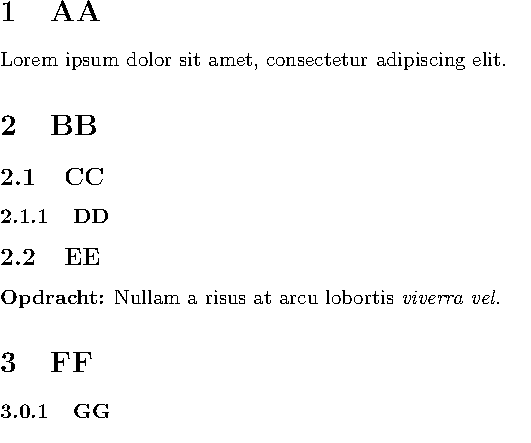
\includegraphics[width=\linewidth,height=0.8\textheight,keepaspectratio]{assets/outdir/simpleContents.pdf}
% 		\end{column}
% 	\end{columns}
% \end{frame}

\begin{frame}
	\frametitle{Veelgebruikte packages}

	\begin{tabularx}{\textwidth}{X l}
		\toprule
		Package & Verbeteringen voor\\
		\midrule
		amsmath & Wiskunde \\
		amssymb & Wiskunde \\
		graphicx & Afbeeldingen \\
		geometry & Pagina marges en grootte (\textbf{a4paper!!!})\\
		xcolor & Kleuren \\
		hyperref & Pdf-navigatie \\
		parskip & Alinea's\\
		babel & Vertalingen\\
		\bottomrule
	\end{tabularx}
	\medskip

	Template op Vincents website: \href{https://vkuhlmann.com/latex/example}{\ul{\texttt{vkuhlmann.com/latex/example}}}
\end{frame}

\begin{frame}
	\frametitle{Subscript/superscript: Inzichtsvragen}

	\emph{Wat mist hier?} \hll|\\vec\{F\}_\{tot\}|
	
	\pause
	Antwoord: de `tot' wordt niet als tekst gezien: $ \vec{F}_{tot} $

	Juiste manier: \hll|\\vec\{F\}_\{\\text\{tot\}\}|, geeft $ \vec{F}_{\text{tot}} $

	\medskip

	\pause
	\emph{Wat gaat hiermee fout?} \hll|\\vec\{F_\{\\text\{tot\}\}\}|

	\pause Hint: \hll|\\vec\{abc\}| = $ \vec{abc} $

	\pause Antwoord: $ \vec{F_{\text{tot}}} $ \uncover<+->{(\hll|\\vec\{F_\{\\text\{tot\}\}\}|)}

	Juiste manier: \uncover<.->{$ \vec{F}_{\text{tot}} $} \uncover<.->{(\hll|\\vec\{F\}_\{\\text\{tot\}\}|)}

	\medskip

	\pause
	\emph{Wat is het verschil tussen \textnormal{\hll|x_0^2|} en \textnormal{\hll|\{x_0\}^2|}?}

	\pause Hint: \hll|x_0^2| = $ x_0^2 $

	\pause Antwoord: Superscript is nu van hele groep, niet alleen van $ x $: $ {x_0}^2 $.

\end{frame}

\section{Typesetting}

\importslide{text}{text-lists.tex}

\begin{frame}
	\frametitle{Lijsten}

	TODO

	% TODO Frames about Description
	
	\begin{description}
		\item AA
		\item[BB] CC
		\item[DD] EE 
	\end{description}
\end{frame}

\importslide{text}{text-quotes.tex}

\section{Figuren}

% \addtorecentlist{\textbackslash includegraphics}

\importslide{images}{includegraphics-asparagraph.tex}
\importslide{images}{includegraphics-center.tex}
\importslide{images}{includegraphics-figure.tex}

\importslide{images}{figure-placement.tex}
\importslide{images}{figure-dimensions.tex}

\importslide{images}{subfigure.tex}

\section{Referenties}

\begin{saveblock}{refWrong}
	\begin{highlightblock}[gobble=8,linewidth=\textwidth,
		framexleftmargin=0.25em,xleftmargin=0.25em]
		Zie pinguin in Figuur 1.
		\begin{figure} % <-- Figuur 1
			... % Pinguin
		\end{figure}
	\end{highlightblock}
\end{saveblock}

\begin{saveblock}{refWrong2}
	\begin{highlightblock}[gobble=8,linewidth=\textwidth,
		framexleftmargin=0.25em,xleftmargin=0.25em]
		\begin{figure} % <-- Figuur 1
			... % Man in tuxedo-pak
		\end{figure}
		Zie pinguin in Figuur 1.
		\begin{figure} % <-- Figuur 2
			... % Pinguin
		\end{figure}
	\end{highlightblock}
\end{saveblock}

\begin{frame}
	\frametitle{Referenties}

	\unless\ifishandout
	\only<1>{\useblock{refWrong}}
	\fi

	\only<2->{\useblock{refWrong2}}
\end{frame}

\begin{saveblock}{refCorrect}
	\begin{highlightblock}[gobble=8,linewidth=\textwidth,
		framexleftmargin=0.25em,xleftmargin=0.25em]
		\begin{figure} % <-- Figuur 1
			... % Man in tuxedo-pak
		\end{figure}
		Zie pinguin in Figuur \ref{fig:pinguin}.
		\begin{figure} % <-- Figuur 2
			... % Pinguin
			\caption{...}\label{fig:pinguin}
		\end{figure}
	\end{highlightblock}
\end{saveblock}

\begin{frame}
	\frametitle{Referenties}

	\useblock{refCorrect}
\end{frame}

\begin{frame}
	\frametitle{Referenties}

	Equation
\end{frame}

\begin{frame}
	\frametitle{Referenties}

	Section
\end{frame}

\begin{frame}
	\frametitle{\texorpdfstring{\LaTeX}{LaTeX}'s systeem voor referenties}


	
\end{frame}

\section{Documentstructuur}

\importslide{document}{document-parts.tex}

\importslide{document}{document-margins.tex}

\importslide{document}{document-sections.tex}

\importslide{document}{document-toc.tex}

\importslide{document}{document-secnumdepth.tex}

\importslide{document}{document-section_star.tex}

\importslide{document}{document-hyperref.tex}


\begin{frame}
	Fancyhdr
\end{frame}

\definecolor{darkred}{rgb}{0.55, 0.0, 0.0}
\definecolor{darkpastelred}{rgb}{0.76, 0.23, 0.13}
\definecolor{darkpastelgreen}{rgb}{0.01, 0.75, 0.24}

\begin{saveblock}{kvlistOverLines}
	\begin{highlightblock}
		\includegraphics[
			width=   0.9 \textwidth
		]{afbeelding.jpg}
	\end{highlightblock}
\end{saveblock}

\begin{saveblock}{kvlistOverLinesParBroken}
	\begin{highlightblock}
		\includegraphics[
			width=   0.9 \textwidth

		]{afbeelding.jpg}
	\end{highlightblock}
\end{saveblock}

\begin{frame}
	\frametitle{Spaties en overzichtelijke code: de verkeersregels}

	\textbf{\textcolor{darkpastelred}{Nope}}: \hll|\\includegraphics[width=0.9\\textwidth]\{| \hll| afbeelding.jpg \}|
	\medskip

	\textbf{\textcolor{darkpastelgreen}{Ok}}
	\useblock{kvlistOverLines}
	\medskip

	\textbf{\textcolor{darkpastelred}{Nope}}
	\useblock{kvlistOverLinesParBroken}
\end{frame}

\begin{saveblock}{packages}
	\begin{highlightblock}
		\usepackage{
			parskip,
			hyperref
		}
	\end{highlightblock}
\end{saveblock}

\begin{saveblock}{indentation}
	\begin{highlightblock}
		\begin{center}
			AA
		\end{center}
		\begin{center}
		BB
		\end{center}
		\begin{center}CC\end{center}
	\end{highlightblock}
\end{saveblock}


\begin{frame}
	\frametitle{Spaties en overzichtelijke code: de verkeersregels}

	\textbf{\textcolor{darkpastelgreen}{Ok}}
	\useblock{packages}
	\medskip

	\textbf{\textcolor{darkpastelgreen}{Ok}}
	\useblock{indentation}
\end{frame}


\begin{frame}
	\frametitle{Stellingen en lemma's}

	TODO
\end{frame}

\begin{frame}
	\frametitle{Tabellen}

	TODO
\end{frame}

\section{\texorpdfstring{}{Misc}}

\importslide{misc}{misc-contact.tex}

\begin{frame}
	\frametitle{Volgende keer -- Week 3 (di 12 okt): Verdiepend}

	\begin{multicols}{2}
		\begin{itemize}
			\item AA
			\item BB
			\item Meer
		\end{itemize}\par
		\vfill
		\leavevmode
	\end{multicols}

	(Voorbeeld van wat je bereikt is te vinden op)
	\begin{center}
		\href{https://a-eskwadraat.nl/latex}{\ul{\texttt{a-eskwadraat.nl/latex}}}
	\end{center}

	\medskip
	Inschrijven nog mogelijk!
\end{frame}

\begin{frame}
	Oefeningen!
\end{frame}

\ifishandout
	\importslide{misc}{misc-license.tex}
\fi
	
\end{document}
